\documentclass[Tesi.tex]{subfiles}

\begin{document}

\section{INTRODUZIONE}
Il debugging indica l'attività che consiste nell'individuazione e correzione da parte del programmatore di uno o più errori (bug) rilevati nel software.
Essa è una delle attività più costose nell’ambito dello sviluppo software, sia in tempo che in termini economici, tale che miglioramenti in questo campo generano un notevole impatto sul piano pratico.
Un debugger è uno strumento software specifico utilizzato per eseguire l'attività di debugging, consentendo l'esecuzione del programma a piccoli passi fino a punti scelti dal programmatore (settando un breakpoint per esempio), mostrando nel contempo lo stato del programma: quali variabili sono in gioco, lo stack di esecuzione ecc..

Secondo una ricerca recente \cite{devops} (2020) di Undo, un'azienda che si occupa di debugging reversibile, in collaborazione con un progetto MBA della Cambridge Judge Business School, emerge che 620 milioni di ore di sviluppo all'anno, in tutto il mondo, vengano impiegate per il debug di errori software, a un costo di circa 61 miliardi di dollari.
Sempre secondo il rapporto emesso, il 41\% degli intervistati ha affermato di aver identificato la riproduzione di un bug come la più grande barriera per trovare e correggere i bug più velocemente, seguita dalla correzione effettiva del bug (23\%). Ben più della metà (56\%) ha affermato che potrebbe rilasciare software uno o due giorni più velocemente se la riproduzione degli errori non fosse un problema. 
Un secondo studio \cite{MBA}, meno recente(2013), eseguito sempre da MBA Cambridge, evidenzia come l’utilizzo della tecnologia di \textit{debug reversibile} permetta un aumento dell'efficienza sul tempo di debugging del 26\%.

Il paradigma di computazione reversibile prevede che i programmi possano essere eseguiti non solo in avanti, bensì anche all'indietro. Ciò permette di recuperare gli stati passati del programma, capacità utile soprattutto nel caso in cui si verifichino errori, in modo tale da procedere successivamente in uno stato di computazione privo di errori.
Nel debugging non reversibile, si sfrutta la combinazione di punti di interruzione (BreakPoint), punti di controllo (ControlPoint) e altri elementi generici di debugging, che fungono da indicatori per aiutare a trovare il bug nel software. Con questi debugger risulta così possibile eseguire il programma finché non raggiunge un punto di interruzione e analizzare eventuali problemi che si verificano in  quella particolare sezione di codice. In alcuni casi, questo approccio funziona perfettamente, ma il più delle volte, non si sa in quale sezione del codice è avvenuto l'errore e se si sa, non si sanno le conseguenze all'interno di questa sezione che generano il bug.
La reversibilità, applicata al debugging, permette la simulazione dell'esecuzione del codice in entrambe le direzioni, \textit{dando la possibilità di soffermarsi in un intorno specifico del codice, al fine di isolare al meglio l'errore, le cause e le conseguenze di quest'ultimo}, cosa che migliora l'attività di debugging, come si evince dallo studio \cite{MBA}.

In questa tesi, il debugging reversibile sarà applicato al linguaggio \textit{Erlang}\cite{erlangDoc}.
Erlang è un linguaggio di programmazione ad attori funzionale, concorrente e distribuito a typing dinamico, basato sulla macchina virtuale BEAM.
Fu progettato per gestire applicazione real-time, 1)fault-tolerant, 2)distribuite e 3)non-stop.
Queste feature, in un'applicazione scritta in Erlang, vengono raggiunte rispettivamente grazie a:
\begin{enumerate}
	\item Link tra i processi, suddividendoli in processi worker e processi supervisor, in cui un supervisor linkato ad un worker, cattura e gestisce \textit{la fine dell'esecuzione del worker}, sia essa la terminazione normale del codice o un'uscita anomala.
	\item API per lo spawn di nodi e processi su nodi, su altre macchine in rete.
	\item Loading del codice a caldo.
\end{enumerate}
L'unità di computazione base del linguaggio Erlang è il processo, come per Java o Python risulta essere 
la classe (più precisamente un oggetto che istanzia una classe).
Questi processi vengono schedulati da BEAM, come un normale sistema operativo, tramite uno scheduler di tipo \textit{preemptive} con politica basata sulle \textit{riduzioni}, ovvero ogni operazione fatta da un processo costa un \textit{certo ammontare di riduzioni}, e raggiunta la soglia limite, viene schedulato un altro processo\footnote{il costo di un operazione in riduzioni dipende da una stima che viene fatta da BEAM, e può variare da esecuzione ad esecuzione}.
I vari processi attivi in un sistema run-time Erlang comunicano attraverso, e solamente così, il \textit{message-passing asincrono}, dato che essi sono totalmente isolati dagli altri processi in esecuzione (ecco perchè si chiamano processi e non thread).
Ogni processo possiede una local mailbox che è implementata da una coda in cui i messaggi inviati da altri processi vengono immagazzinati, in attesa di essere elaborati.
\textbf{\textit{Il motivo per cui è stato scelto Erlang come linguaggio di riferimento risiede nel fatto che la parte sequenziale e la parte concorrente del linguaggio sono ben distinguibili fra di loro}}.

Attualmente, il debug reversibile per linguaggi sequenziali è ben compreso e ha trovato applicazioni in ambito industriale.
Tuttavia, oggigiorno la maggior parte del software, soprattutto in ambito web, si sta spostando verso il paradigma concorrente, dato l'avvento di cpu multi-core in primis. Sfortunatamente, la nozione di reversibilità in un contesto concorrente è intrinsecamente diversa dalla nozione di reversibilità in un contesto sequenziale.
In un contesto sequenziale, l'ultimo stato di un programma è individuabile nello \textit{stato del programma alla penultima riga di codice}, mentre in ambito concorrente, non è mai ben definita l'ultima riga di codice, come si nota nell'esempio \ref{seqconc}, dato che l'esecuzione di un codice concorrente, ripetuto più volte con gli stessi input, può variare di volta in volta, quando nell'ambito sequenziale è sempre univocamente definito il flusso di codice per gli stessi input.
Nello specifico di Erlang, l'esecuzione temporale del codice può sovrapporsi tra i vari processi, dato che  la macchina virtuale BEAM\cite{smp}, \textit{per ogni core della cpu}, crea un \textit{thread scheduler}, che gestisce una coda di processi Erlang, ottendo la \textit{concorrenza reale} della computazione.
Sono possibili due soluzioni:
\begin{itemize}
	\item Sequenzializzazione dell'esecuzione del codice.
	\item Si trova una nozione differente di reversibilità per la programmazione concorrente. 
\end{itemize}
\subfile{./Introduzione/EsempioSeqConc/esempio}
Si consideri inoltre che, con l'approccio di programmazione concorrente, si aggiungono, nel programma, tipi di bug intrinsechi ad esso, quali \textit{deadlock}, \textit{race conditions} o \textit{starvation}.
Seppur i linguaggi di programmazione basati sul paradigma concorrente evitino questi tipi di bug a livello di progettazione, \textbf{tramite politiche ben definite e scelte durante la progettazione del linguaggio}\footnote{Nello specifico di Erlang, se si verifica un deadlock, BEAM uccide i processi coinvolti in esso, per poi farli ripartire uno alla volta, ed effettuando dei controlli su di essi.}, si può comunque incorrere in altri tipi di bug, relativi alla concorrenza, durante lo sviluppo software con questi linguaggi, uno in particolare relativo ad Erlang, quale la \textit{violazione dell'ordine di invio dei messaggi}.\footnote{Ipotizziamo di avere due processi X e Y rispettivamente sender e receiver. X invia z al tempo T=1 ed al tempo T=2 invia q. Non è detto che arrivi prima z di q, nonostante fosse stato inviato prima.}
\textbf{Nello specifico per Erlang, la sequenzializzazione fallisce in principio in cpu multi-core, ma in generale essa risulta essere totalmente inefficiente per il paradigma concorrente in quanto, la sequenzializzazione, oltre ad avere un grosso overhead, tralascia le \textit{informazioni relative alla causalità}. Quest'ultime risultano essere fondamentali e centrali in relazione ai bug sopra citati, e in generale ai bug nella concorrenza, in quanto questi bug posso apparire in una esecuzione ma non apparire in un esecuzione successiva dello stesso codice, dipendendo dalla velocità di esecuzione dei singoli processi e da come questi interagiscano tra di loro}.
In figura \ref{bug}, un sender (\textit{sender}) invia due numeri (2,0) a due diversi intermediari (\textit{inter}), che a loro volta invieranno i loro numeri ad un worker (\textit{worker}), che effettuerà una divisione. In base alla sequenza di arrivo di questi due numeri, il worker può restituire 0 o andare in errore, e questa sequenza di arrivo non è mai univoca, anzi varia in base \textit{allo scheduling}.
\subfile{./Introduzione/EsempioBug/esempio}
Tutto ciò porta alla ricerca di una nozione di reversibilità alternativa per la programmazione concorrente.
Anticipo che questa nozione di reversibilità sarà la reversibilità \textit{causal-consistent} \cite{causal}, ovvero una nozione che non si basa sul concetto di tempo, bensì sul concetto di \textit{causalità} tra gli eventi.
Questo concetto specifica \underline{quali} azioni possono essere annullate.
Questa nozione verrà approfondita nel capitolo relativo al background.

Al momento l'unico debugger reversibile per Erlang che sfrutta la nozione sopracitata di reversibilità è Cauder, che è scritto esso stesso in Erlang (link: \href{https://github.com/mistupv/cauder}{https://github.com/mistupv/cauder}).
Allo stato dell'arte, Cauder supporta solo alcune primitive del linguaggio Erlang, quali, in relazione alla parte concorrente, la \textit{spawn}, per la creazione di nuovi processi, e la \textit{send}, per l'invio di messaggi, mentre per la parte sequenziale, la \textit{self}, che ritorna il pid del processo che la chiama, e la \textit{sleep}, che sospende il processo chiamante.
\textbf{Molto importante, Cauder gestisce un solo thread scheduler}.
In realtà Cauder non lavora direttamente sul codice sorgente puro di Erlang, bensì su un linguaggio di compilazione intermedio tra Erlang e BEAM, il Core Erlang\cite{coreErlang}.
La scelta di utilizzare Core Erlang invece che Erlang puro, risiede nel fatto che, esistono, nella libreria standard Otp di BEAM, packages che permettono la compilazione di moduli Erlang in questo linguaggio e la manipolazione diretta del codice risultante dopo questa compilazione, tramite strutture dati(tuple/mappe), risultando nel contempo essere un linguaggio abbastanza simile ad Erlang puro.

Cauder permette di eseguire un programma, dopo averlo caricato e compilato dal menù a tendina File, in 3 modalità:
\begin{itemize}
	\item Manuale: si sceglie un Pid/MessageId e si manda avanti o indietro di un passo il processo/messaggio.
	\item Automatica: si sceglie un numero N di passi e il sistema avanza o torna indietro, se possibile, di N passi, \textit{secondo uno scheduling ben definito}.
	\item Rollback: una particolare funzionalità che permette di fare \textit{l'undo di una specifica azione compiuta da un processo o un messaggio, incluse tutte le sue conseguenze}. 
\end{itemize}
\begin{figure}[H]
\centerline{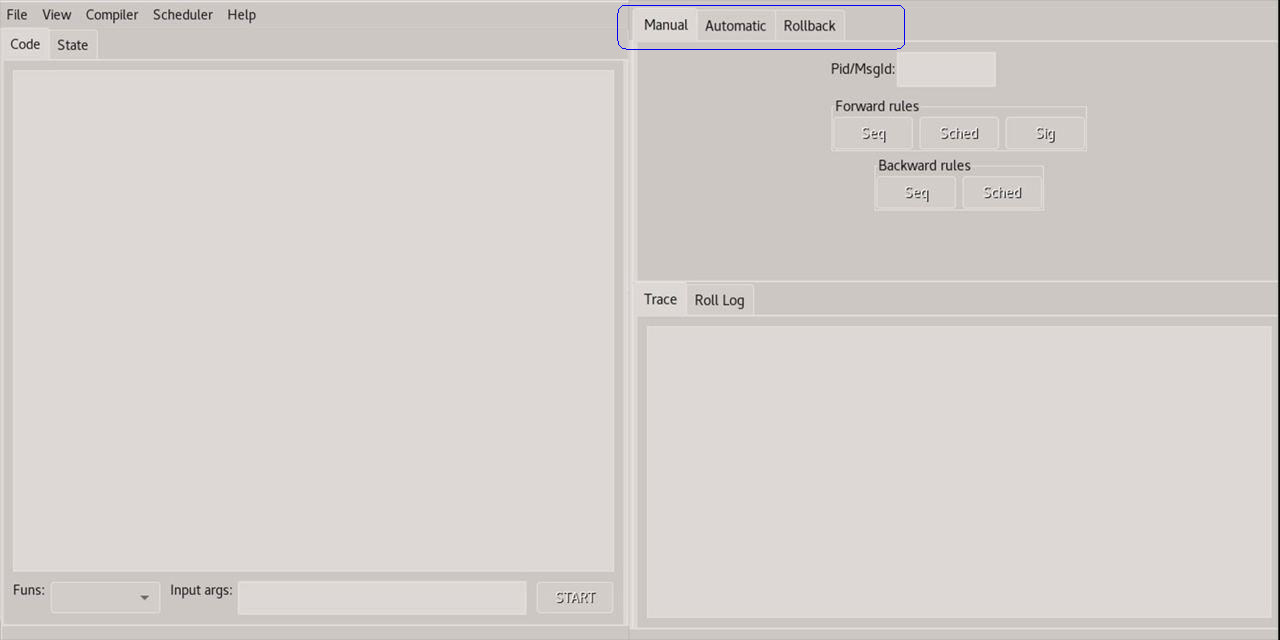
\includegraphics[scale=0.4]{./Files/CauderPanoramica}}
\caption{La finestra iniziale di Cauder}
\label{fig1}
\end{figure}
Questa tesi verte su \textit{un'estensione} di Cauder, tramite l'implementazione dei \textit{link e la gestione della terminazione del codice}, per la gestione degli errori.\\
Ciò che introdurrò in primis sarà la nozione di reversibilità in generale, una nozione di reversibilità che si adatta alla nozione di concorrenza e infine l'applicazione di essa al debugging.\\
Successivamente illustrerò il linguaggio di Cauder, le strutture dati che manipola e le regole informali che implementa e come esse fanno evolvere le strutture dati gestite da Cauder.\\
Infine passerò ad illustrare l’implementazione dell’estensione del linguaggio supportato, ovvero come esso viene esteso, le strutture dati estese di  Cauder e come evolvono, secondo le nuove regole semantiche derivanti dalla gestione degli errori e i link a run time.
\end{document}
